\subsection{Kombinační čísla}
\label{ssec:kombinacni-cisla}

V této sekci se budeme zabývat asi poměrně přirozenou otázkou -- kolik má
množina $X$ podmnožin velikosti $k$, kde $k$ může být libovolné číslo od $0$ do
$\# X$. Pro $k=0$ i $k=\# X$ je odpověď jednoduchá: přesně jednu. Pro $k = 1$
člověku hádám taky dojde, že jednoprvková podmnožina je vlastně totéž, co její
jediný prvek, takže takových máme $\# X$. Od $k = 2$ nám ale začína, borcovia,
prituhovať. Nejspíš bychom pořád zvládli počet dvouprvkových množin nějak
zpatlat, ale co třeba $k = \# X / 2$ (když je $\# X$ sudé) a podobné takřka
nekřesťanské výmysly? To už chce nějaké udělátko.

Nejdřív si to ale, jakožto slušní a spořádaní matematikové, definujeme.

\begin{definition}[Počet $k$-prvkových podmnožin]
 Ať $X$ je množina a $0 \leq k \leq \# X$ je přirozené číslo. Definujeme množinu
 \[
  \binom{X}{k} \coloneqq \{A \subseteq X \mid \# A = k\}
 \]
 všech $k$-prvkových podmnožin množiny $X$. Výraz $\binom{X}{k}$ čteme \uv{$X$ 
 nad $k$}.
\end{definition}

Chvilku se budeme bavit přemítáním o způsobu, jak spočítat $\# \binom{X}{k}$ pro
libovolné $k$ mezi $0$ a $\# X$.

Použijeme kombinatorickou metodu důkazu zvanou \emph{počítání dvěma způsoby}.
Jde o užitečný (a podle mého velmi elegantní) přístup ve chvíli, kdy neumím
spočítat rovnou konkrétní množství, ale umím spočítat něco vel\-mi podobného.
Technika počítání dvěma způsoby spočívá v tom, že tu kvantitu, kterou spočítat
\emph{umím}, vyjádřím na jedné straně pomocí kvantity, kterou spočítat
\emph{neumím}, a na druhé straně pomocí vzorečku, který znám. To mi dá rovnici,
ze které pak vyjádřím to číslo, které chci určit.

Takto abstraktně vám asi \emph{počítání dvěma způsoby} nic neřeklo, takže je
raději pojďme aplikovat na zpytovaný problém. Počet $k$-prvkových podmnožin $X$
spočítat neumím; což takhle začít tím, že si nějakou náhodnou podmnožinu
$\{x_1,\ldots,x_k\} \subseteq X$ zvolím. Jeden z důvodů, proč neumím počet
takovýchhle podmnožin spočítat, je, že mi chybí nějaké \emph{uspořádání}.

Zatím všechny věci, které jsme počítali, byly v jistém smyslu \emph{uspořádané}.
Počet všech zobrazení $A \to B$ jsme počítali tak, že jsme prvky $A$
\textbf{jeden po druhém} zobrazovali na prvky $B$. Vlastně nevědomky jsme si tak
nějakým náhodným způsobem \emph{uspořádali} množinu $A$, aby se nám dobře
počítalo. Permutace jsou taky přímo definované tak, že mění \emph{uspořádání}
prvků na množině.

Vybrat si nějaké uspořádání na $X$ a všechny její podmnožiny pak považovat za
uspořádané podle stejného uspořádání je chytrý nápad, který přinese ovoce. Na
konci výpočtu je však potřeba zanedbat všechny možné způsoby, kterými jsme 
$k$-prvkové množiny mohli uspořádat. Uvidíte, že nám nakonec opravdu vyjde, že
počet všech $k$-prvkových podmnožin $X$ je vlastně počet všech $k$-prvkových
podmnožin $X$ s nějakým konkrétním uspořádáním dělen počtem způsobů, kolika jsme
takové uspořádání mohli zvolit.

Pojďme tedy místo množiny $\{x_1,\ldots,x_k\}$ uvažovat její \uv{uspořádanou
verzi}, tím míním $k$-tici $(x_1,\ldots,x_k)$. Rozdíl je samozřejmě v tom, že
(třeba pro $k = 3$) je množina $\{x_1,x_2,x_3\}$ ta samá, co $\{x_2,x_1,x_3\}$,
ale trojice $(x_1,x_2,x_3)$ je různá od trojice $(x_2,x_1,x_3)$. Záleží na
pořadí, v jakém prvky za sebe umisťuji, na \emph{uspořádání}.

Na první straně rovnice vzniklé \emph{počítáním dvěma způsoby} si určíme, kolik
různých takových $k$-tic mi z jedné množiny může vzniknout. No přeci tolik,
kolika způsoby mohu mezi sebou proházet (nebo třeba cizeji \uv{pro\-permutovat}
$\leftarrow$ hint btw) její prvky. Každá permutace na $\{x_1,\ldots,x_k\}$ mi
určuje přesně jedno možné uspořádání. Těch je, podle
\hyperref[prop:pocet-permutaci-na-mnozine]{tvrzení~\ref*{prop:pocet-permutaci-na-mnozine}},
$k!$. Z~definice máme $\# \binom{X}{k}$ různých $k$-prvkových podmnožin $X$ a
každá určuje $k!$ uspořádaných $k$-tic. Celkem těchto tedy máme $k! \cdot \#
\binom{X}{k}$. To činí jednu stranu naší rovnice.

Na druhé straně, vybrat $k$ prvků z $X$ a nějak je uspořádat je přeci to samé,
jako jim nějak přiřadit čísla od $1$ do $k$. Takovéhle přiřazení mi určí přesně,
v jakém pořadí prvky $x_1,\ldots,x_k$ jsou. Tedy, ten prvek, který dostane $1$,
jde první, ten s $2$ jde druhý atd.

Uvědomme si, že výběr přesně $k$ prvků z množiny $X$ a jejich následné
uspořádání (tedy přiřazení čísel od $1$ do $k$) je vlastně prosté zobrazení ${f:
\{1,\ldots,k\} \to X}$. Každému takovému zobrazení odpovídá uspořádaná $k$-tice
$(f(1),\ldots,f(k))$ prvků z $X$ a naopak každou $k$-tici $(x_1,\ldots,x_k)$
lze považovat za prosté zobrazení $g: \{1,\ldots,k\} \to X$ takové, že
$g(i)=x_i$ pro všechna $i \leq k$. Čili, pro každou podmnožinu
$\{x_1,\ldots,x_k\} \subseteq X$ mám tolik uspořádaných $k$-tic
$(x_1,\ldots,x_k)$ jako mám prostých zobrazení $\{1,\ldots,k\} \to X$. Podle
\hyperref[claim:pocet-prostych-zobrazeni]{tvrzení~\ref*{claim:pocet-prostych-zobrazeni}}
je tento počet roven $\prod_{i=0}^{k-1} \#X-i$.

Na závěr již stačí obě množství vzniklá dvěma různými způsoby počítání
uspořádaných $k$-prvkových podmnožin $X$ porovnat. Dostaneme
\[
 \prod_{i=0}^{k-1} \# X-i = k! \cdot \# \binom{X}{k}, 
\]
odkud okamžitě plyne
\[
 \# \binom{X}{k} = \frac{\prod_{i=0}^{k-1} \# X - i}{k!}.
\]

Diskuse tvořící obsah předchozích dvou stránek je velmi obšírným důkazem
následujícího tvrzení.

\begin{claim}[Počet $k$-prvkových podmnožin]
 \label{claim:pocet-k-prvkovych-podmnozin}
 Ať $X$ je konečná množina. Pak počet všech $k$-prvkových podmnožin $X$ je roven
 \[
  \frac{\prod_{i=0}^{k-1} \# X - i}{k!}.
 \]
\end{claim}

K tomuto tvrzení se víže definice tzv. \emph{kombinačního čísla}.

\begin{definition}[Kombinační číslo]
 \label{def:kombinacni-cislo}
 Ať $k,n \in \N$ a $k \leq n$. Pak definujeme
 \[
  \binom{n}{k} \coloneqq \frac{\prod_{i=0}^{k-1} n-i }{k!}.
 \]
 Výraz $\binom{n}{k}$ čteme $n$ nad $k$.
\end{definition}

V závěsu \hyperref[def:kombinacni-cislo]{definice~\ref*{def:kombinacni-cislo}}
můžeme
\hyperref[claim:pocet-k-prvkovych-podmnozin]{tvrzení~\ref*{claim:pocet-k-prvkovych-podmnozin}}
přepsat jako rovnost
\[
 \# \binom{X}{k} = \binom{\# X}{k}.
\]

Ve škole se často učí interpretace kombinačního čísla $\binom{n}{k}$ jako
\uv{počet způsobů, jak volit $k$ předmětů z $n$ bez závislosti na pořadí}. Ta je
plně v souladu s naší definicí, interpretujeme-li $X$ jako množinu předmětů a
jednu její $k$-prvkovou podmnožinu jako výběr $k$ předmětů, kde však
pochopitelně (jedná se o \textbf{podmnožinu}) nezáleží na jejich uspořádání.

\subsubsection{Problém rozkladu na sčítance}
\label{sssec:problem-rozkladu-na-scitance}

Oblíbený problém, který lze řešit počítáním způsobů, jak volit počet sourodých
předmětů z většího množství, ale nikdo by to na první pohled nečekal, je
\emph{problém rozkladu na sčítance}.

Volme číslo $m \in \N$. \emph{Rozkladem čísla $m$ na $r$ sčítanců} myslíme
rovnost
\[
 m = x_1 + x_2 + \cdots + x_r = \sum_{k=1}^{r} x_k,
\]
kde $x_i \geq 0$ jsou nezáporná celá čísla. Zajímá nás, kolika způsoby lze dané
číslo $m$ rozložit na $r$ (ne nutně různých) sčítanců. Na první pohled nejde
vůbec o kombinace (tedy o výběr bez závislosti na pořadí), protože pořadí
sčítanců je zde důležité: rozklad $7 = 0 + 2 + 5$ \textbf{je různý} od rozkladu
$7 = 2 + 0 + 5$. Situace se navíc v tomto směru zdá zcela beznadějná, neboť když
jsou dvě a více čísel v rozkladu stejná, pak jejich prohození samozřejmě
neurčuje jiný rozklad. Například, v rozkladu $7 = 2 + 2 + 3$ mohu prohodit první
$2$ s druhou $2$ a nedostat tak odlišný rozklad.

První průlomovou myšlenkou je náhled, že číslo $m$ vlastně \uv{rozhazuji} mezi
$r$ čísel. V tomto smyslu si lze představit přirozené číslo $m$ jako $m$
nerozlišitelných míčků, které rozděluji do $r$ košíků. Třeba rozklad $7 = 0 + 2
+ 5$ by vypadal takto.

\begin{figure}[h]
 \centering
 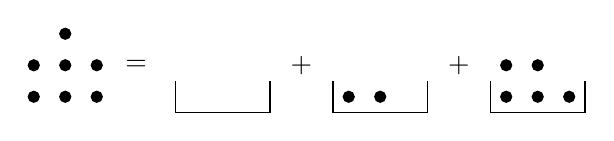
\begin{tikzpicture}
  \foreach \i in {-0.4,0} {
   \foreach \j in {0,0.4,0.8} {
    \draw[fill=black]  (\j, \i) circle (2pt);
   }
  }
  \draw[fill=black] (0.4, 0.4) circle (2pt);

  \node at (1.3, 0) {$=$};

  \foreach \j in {0,0.4} {
   \draw[fill=black]  (4 + \j, -0.4) circle (2pt);
  }

  \draw (1.8, -0.2) -- (1.8,-0.6);
  \draw (1.8, -0.6) -- (3,-0.6);
  \draw (3, -0.6) -- (3,-0.2);

  \node at (3.4,0) {$+$};

  \draw (3.8, -0.2) -- (3.8,-0.6);
  \draw (3.8, -0.6) -- (5,-0.6);
  \draw (5, -0.6) -- (5,-0.2);

  \node at (5.4,0) {$+$};

  \foreach \j in {0,0.4,0.8} {
   \draw[fill=black]  (6 + \j, -0.4) circle (2pt);
  }
  \draw[fill=black]  (6, 0) circle (2pt);
  \draw[fill=black]  (6.4, 0) circle (2pt);

  \draw (5.8, -0.2) -- (5.8,-0.6);
  \draw (5.8, -0.6) -- (7,-0.6);
  \draw (7, -0.6) -- (7,-0.2);
 \end{tikzpicture}
 \label{fig:micky-do-kosiku}
 \caption{Vizualizace rozkladu $7 = 0 + 2 + 5$ jako rozdělení míčků do košíků.}
\end{figure}

Samozřejmě, v takovémto rozkladu určuje pravá strana jednoznačně tu levou, takže
není třeba $7$ míčků na levé straně znázorňovat. Podobně, když se dohodneme, že
počty míčků v košících vždy sčítáme, lze i symboly $+$ vynechat. Trochu
složitější rozklad, třeba $9 = 1 + 0 + 3 + 5$ bychom nakreslili jak vidno na
\hyperref[fig:jenom-micky-a-kosiky]{obrázku~\ref*{fig:jenom-micky-a-kosiky}}.

\begin{figure}[h]
 \centering
 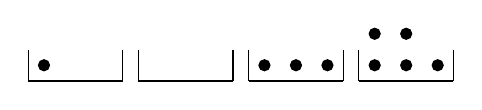
\begin{tikzpicture}
  \foreach \k in {0} {
   \draw (\k,-0.2) -- (\k,-0.6);
   \draw (\k,-0.6) -- (\k+1.2,-0.6);
   \draw (\k+1.2,-0.6) -- (\k+1.2,-0.2);
  }
  \draw[fill=black]  (0.2, -0.4) circle (2pt);

  \foreach \k in {1.4} {
   \draw (\k,-0.2) -- (\k,-0.6);
   \draw (\k,-0.6) -- (\k+1.2,-0.6);
   \draw (\k+1.2,-0.6) -- (\k+1.2,-0.2);
  }

  \foreach \k in {2.8} {
   \draw (\k,-0.2) -- (\k,-0.6);
   \draw (\k,-0.6) -- (\k+1.2,-0.6);
   \draw (\k+1.2,-0.6) -- (\k+1.2,-0.2);
  }
  \foreach \j in {0,0.4,0.8} {
   \draw[fill=black]  (3 + \j, -0.4) circle (2pt);
  }

  \foreach \k in {4.2} {
   \draw (\k,-0.2) -- (\k,-0.6);
   \draw (\k,-0.6) -- (\k+1.2,-0.6);
   \draw (\k+1.2,-0.6) -- (\k+1.2,-0.2);
  }
  \foreach \j in {0,0.4,0.8} {
   \draw[fill=black]  (4.4 + \j, -0.4) circle (2pt);
  }
  \foreach \j in {0,0.4} {
   \draw[fill=black]  (4.4 + \j, 0) circle (2pt);
  }
 \end{tikzpicture}
 \caption{Zjednodušený nákres rozdělení míčků do košíků.}
 \label{fig:jenom-micky-a-kosiky}
\end{figure}

Nakonec si uvědomíme, že přeci není ani třeba kreslit jednotlivé košíky. Stačí,
když všechny míčky vysypeme na zem a jenom mezi ně dáme nějaká hradla, abychom
věděli, které míčky patřily do stejného košíku. Názorná ukázka, pro stejný
rozklad, tedy $9 = 1 + 0 + 3 + 5$.

\begin{figure}[h]
 \centering
 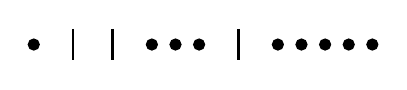
\begin{tikzpicture}
  \draw[fill=black] (0, 0) circle (2pt);
  \draw[thick] (0.5, 0.2) -- (0.5, -0.2);
  \draw[thick] (1, 0.2) -- (1, -0.2);
  
  \foreach \i in {0,0.3,0.6} {
   \draw[fill=black] (1.5 + \i, 0) circle (2pt);
  }

  \draw[thick] (2.6, 0.2) -- (2.6, -0.2);
  \foreach \i in {0,0.3,...,1.5} {
   \draw[fill=black] (3.1 + \i, 0) circle (2pt);
  }
 \end{tikzpicture}
 \caption{Ještě jednodušší nákres rozkladu $9 = 1 + 0 + 3 + 5$.}
 \label{fig:nejjednodussi-micky-s-kosiky}
\end{figure}

Jeden možný způsob, jak si snadno představit spojitost mezi rozkladem a touto
poslední verzí jeho vizualizace je ten, že stěny či hradla odpovídají symbolům
$+$ a počet míčku mezi dvěma hradly odpovídá číslu mezi příslušnými symboly.
Protože sčítanců je $r$, a tedy symbolů $+$ je $r - 1$, je hradel též $r - 1$.

Jsme připraveni řešení úlohy završit. Rozmysleli jsme si, že každé rozmístění $r
- 1$ hradel mezi $m$ za sebou v řadě ležících míčků mi definuje jeden konkrétní
rozklad čísla $m$ na $r$ sčítanců. Stačí tedy umět určit počet takových
rozmístění.

To ale není těžké. Míčky a hradla činí dohromady $m + r - 1$ objektů, z kterých
přesně $r - 1$ jsou hradla. Řečeno jinak, když z $m + r - 1$ objektů vyberu těch
$r - 1$, která se stanou hradly, a zbytek přetvořím v míčky, pak určím rozklad
čísla $m$ na $r$ sčítanců. Počet všech možných výběrů $r - 1$ prvků z~množiny o
$m + r - 1$ prvcích je $\binom{m + r - 1}{r-1}$, kteréžto číslo je tudíž i počet
způsobů, jak rozložit číslo $m$ na $r$ sčítanců.

\subsubsection{Pár vlastností kombinačních čísel}
\label{sssec:par-vlastnosti-kombinacnich-cisel}

Tahle sekce si neklade za cíl objevit zatím neznámý kontinent ani čtenáře naučit
životu v afrických pralesích. Baže naopak, jedná se o prostou přílohu k již
známému. Kombinační čísla se objevují, kdykoli člověk počítá s~podobjekty
konečných objektů, tedy v podstatě pořád. Věnujeme chvilku času prozkoumání
způsobů, jak s nimi zacházet.

Nejprve jeden výpočetně užitečný vzoreček.

\begin{lemma}
 \label{lem:vzorec-pro-kombinacni-cislo}
 Ať $k,n \in \N$, $k \leq n$. Platí
 \[
  \binom{n}{k} = \frac{n!}{k!(n-k)!}.
 \]
\end{lemma}
\begin{proof}
 Z \hyperref[def:kombinacni-cislo]{definice kombinačního čísla} máme
 \[
  \binom{n}{k} = \frac{\prod_{i=0}^{k-1} n-i}{k!},
 \]
 stačí tedy ukázat, že
 \[
  \prod_{i=0}^{k-1} n - i = \frac{n!}{(n-k)!}.
 \]
 To je však zřejmé, neboť
 \begin{align*}
  n! &= n(n-1) \cdots (n-k+1)(n-k)(n-k-1) \cdots 1\\
  &= n(n-1)\cdots (n-k+1)(n-k)! = \left( \prod_{i=0}^{k-1} n-i \right)(n-k)!.
 \end{align*}
 Důkaz plyne z vydělení poslední rovnice číslem $(n-k)!$.
\end{proof}

Dále si povíme o tzv. \emph{Pascalově trojúhelníku}. Tím se obvykle míní
následující struktura.

\begin{figure}[h]
 \centering
 \begin{tikzpicture}
  \node at (0,0.5) {$1$};

  \node at (-0.5,0) {$1$};
  \node at (0.5,0) {$1$};

  \node at (-1,-0.5) {$1$};
  \node at (0,-0.5) {$2$};
  \node at (1,-0.5) {$1$};

  \node at (-1.5,-1) {$1$};
  \node at (-0.5,-1) {$3$};
  \node at (0.5,-1) {$3$};
  \node at (1.5,-1) {$1$};

  \node at (-2,-1.5) {$1$};
  \node at (-1,-1.5) {$4$};
  \node at (0,-1.5) {$6$};
  \node at (1,-1.5) {$4$};
  \node at (2,-1.5) {$1$};

  \node at (-2.5,-2) {$1$};
  \node at (-1.5,-2) {$5$};
  \node at (-0.5,-2) {$10$};
  \node at (0.5,-2) {$10$};
  \node at (1.5,-2) {$5$};
  \node at (2.5,-2) {$1$};

  \node at (0, -2.5) {$\vdots$};
 \end{tikzpicture}
 \caption{Pascalův trojúhelník.}
 \label{fig:pascaluv-trojuhelnik}
\end{figure}

Jde vlastně o posloupnost řad, kde na začátku a na konci každé řady je číslo $1$
a prostřední čísla dostanu tak, že sečtu ta dvě čísla z předchozí řady těsně nad
ním.

Formálně můžeme říci, že Pascalův trojúhelník je posloupnost uspořádaných
$n$-tic $(p_1^{n},\ldots,p_n^{n}) \in \N^{n}$ ($n$ jsou \textbf{indexy} řádků,
nikoli mocniny), taková, že $p_i^{n} = p_{i-1}^{n-1} + p_{i}^{n-1}$ pro každé $n
\geq 1$ a každé $1 \leq i \leq n$. Pro začátek položíme $p_1^{1} = 1$ a v každém
řádku dodefinujeme $p_{0}^{n} = p_{n+1}^{n} = 0$.

Skutečně, když $p_1^{1} = 1$, tedy první číslo prvního řádku je $1$, pak
$p_1^{2} = p_0^{1} + p_1^{1} = 0 + 1 = 1$ a $p_2^{2} = p_1^{1} + p_2^{1} = 1 + 0
= 1$, čili druhý řádek je dvojice $(1, 1)$. Zde vidíte důvod, proč jsme
dodefinovali též $0$-tý a $(n+1)$-ní prvek $n$-tého řádku. Museli bychom totiž
jinak psát speciální pravidlo pro určení prvního a posledního prvku každého
řádku. Místo toho předstíráme, že je Pascalův trojúhelník ještě z obou stran
obklopen nulami.

Pro pořádek si ještě v tomto formálním pohledu spočteme třetí řádek, tj. trojici
$(p_1^{3},p_2^{3},p_3^3)$. Máme
\begin{align*}
 p_1^3&= p_0^2+p_1^2 = 0 + 1 = 1, \\
 p_2^3&= p_1^{2}+p_2^2 = 1 + 1 = 2, \\
 p_3^3&= p_2^2 + p_3^2 = 1 + 0 = 1.
\end{align*}
Vše je, jak má být.

Budeme chtít ukázat, že $n$-tý řádek Pascalova trojúhelníku tvoří přesně čísla
$\binom{n-1}{0},\binom{n-1}{1},\ldots,\binom{n-1}{n-1}$. Pro první řádky je to
jistě pravda, neboť $\binom{0}{0} = 1$ (neboť $0!$ se tradičně definuje jako
$1$) a dále $\binom{1}{0} = \binom{1}{1} = 1$.

Rozepíšeme si, co naše tvrzení vlastně znamená z pohledu kombinačních čísel.
Prvky $p_i^{n+1}$ v $(n+1)$-ním řádku Pascalova trojúhelníku jsou definovány
pomocí prvků v předchozím řádku vzorcem $p_{i+1}^{n+1} = p_{i}^{n} +
p_{i+1}^{n}$. A my tvrdíme, že $p_{i}^{n} = \binom{n-1}{i-1}$. (Ověřte si, že to
je \textbf{opravdu} to, co říkáme!) Přepíšeme-li tuto rovnost v kombinačních
číslech, potřebujeme dokázat, že
\begin{equation*}
 \label{eq:pascal-identity}
 \tag{$*$}
 \binom{n}{i} = \binom{n-1}{i-1} + \binom{n-1}{i}
\end{equation*}
pro každé $n \geq 1$ každé $1 \leq i \leq n$.

I když by to jistě nějak šlo upočítat, my zvolíme elegantnější způsob, který
zůstává věrný tomu, co kombinační číslo vlastně \textbf{vyjadřuje}. Nezapomeňte,
že $\binom{n}{i}$ je počet $i$-prvkových podmnožin $n$-prvkové množiny. Je
jisté, že množina $(i-1)$-prvkových podmnožin je disjunktní (má prázdný průnik) s
množinou $i$-prvkových podmnožin. To ovšem znamená, že
\begin{align*}
 \# \left( \binom{\{1,\ldots,n-1\}}{i-1} \cup \binom{\{1,\ldots,n-1\}}{i}
 \right)
 &= \# \binom{\{1,\ldots,n-1\}}{i-1} + \# \binom{\{1,\ldots,n-1\}}{i}\\
 &= \binom{n-1}{i-1} + \binom{n-1}{i}.
\end{align*}
Řečeno selsky, když vezmu množinu obsahující všechny $i$-prvkové i
$(i-1)$-prvkové podmnožiny, pak její velikost je počet všech $i$-prvkových
podmnožin plus počet všech $(i-1)$-prvkových podmnožin. No shit.

Čili, abychom dokázali rovnost \eqref{eq:pascal-identity}, najdeme bijekci mezi
množinou všech $i$-prvkových a $(i-1)$-prvkových podmnožin $(n-1)$-prvkové
množiny a množinou všech  $i$-prvkových podmnožin $n$-prvkové množiny.

\begin{claim}[Pascalova rovnost]
 \label{claim:pascalova-rovnost}
 Ať $1 \leq i,n \in \N$ a $i \leq n$. Pak platí
 \[
  \binom{n}{i} = \binom{n-1}{i-1} + \binom{n-1}{i}.
 \]
\end{claim}
\begin{proof}
 Definujeme bijekci
 \[ 
  f: \binom{\{1,\ldots,n-1\}}{i-1} \cup \binom{\{1,\ldots,n-1\}}{i} \to
  \binom{\{1,\ldots,n\}}{i}.
 \]
 Ať nejprve $A \in \binom{\{1,\ldots,n-1\}}{i}$, čili $A$ je $i$-prvková
 podmnožina ${\{1,\ldots,n-1\}}$. Pak je $A$ též $i$-prvková podmnožina
 $\{1,\ldots,n\}$, neboli $A \in \binom{\{1,\ldots,n\}}{i}$ a stačí definovat
 $f(A) \coloneqq A$. Stručně řečeno, $f$ je identické zobrazení na $i$-prvkových
 podmnožinách.

 Teď ať $B \in \binom{\{1,\ldots,n-1\}}{i-1}$. Pak $B \cup \{n\}$ je $i$-prvková
 podmnožina $\{1,\ldots,n\}$ a tedy můžeme definovat $f(B) \coloneqq B \cup
 \{n\}$.

 Je zřejmé, že $f$ je bijekce. Když $A \subseteq \{1,\ldots,n\}$ neobsahuje $n$,
 pak je jejím vzorem při $f$ ta samá množina, tj. $A$. Když $A \subseteq
 \{1,\ldots,n\}$ obsahuje $n$, pak je jejím vzorem množina $A \setminus
 \{n\} \subseteq \{1,\ldots,n-1\}$.

 Tím je důkaz dokončen.
\end{proof}

\hyperref[claim:pascalova-rovnost]{Předchozí tvrzení} ukazuje, že pro $n$-tý
řádek Pascalova trojúhelníka oprav\-du platí rovnost
\[
 (p_1^{n},\ldots,p_n^{n}) = \left(
 \binom{n-1}{0},\binom{n-1}{1},\ldots,\binom{n-1}{n-1} \right).
\]

Na závěr celé sekce o kombinačních číslech si ukážeme ještě poslední snadno
dokazatelnou rovnost, která je však výpočetně též užitečná.

\begin{lemma}
 \label{lemma:stejne-doplnku}
 Ať $k,n \in \N$ a $k \leq n$. Pak
 \[
  \binom{n}{k} = \binom{n}{n-k}.
 \]
\end{lemma}
\begin{proof}
 Nalezneme bijekci
 \[
  \binom{\{1,\ldots,n\}}{k} \to \binom{\{1,\ldots,n\}}{n-k}.
 \]
 Uvědomme si, že když $A \subseteq \{1,\ldots,n\}$ a $\# A = k$, pak $\#
 (\{1,\ldots,n\} \setminus A) = n - k$. Kýžená bijekce je tudíž zobrazení $A
 \mapsto \{1,\ldots,n\} \setminus A$.
\end{proof}

Ještě několik úloh pro bystré hlavy.

\begin{exercise}
 Dokažte, že
 \[
  \sum_{i=0}^{n} \binom{n}{i}^2 = \binom{2n}{n}.
 \]
 \textbf{Hint}: použijte
 \hyperref[lemma:stejne-doplnku]{lemma~\ref*{lemma:stejne-doplnku}}.
\end{exercise}

\begin{exercise}
 Dokažte vzorec
 \[
  \sum_{k=r}^{n} \binom{k}{r} = \binom{n+1}{r+1}
 \]
 pro pevné $r \in \N$ indukcí podle $n \in \N$.
\end{exercise}

\begin{exercise}[těžké]
 Kolik existuje podmnožin $\{1,\ldots,n\}$, které neobsahují žádná dvě po sobě
 jdoucí čísla. Formálně, určete velikost množiny
 \[
  \{A \subseteq \{1,\ldots,n\} \mid \{i,j\} \nsubseteq A, \text{ kdykoli }
  |i-j|=1\}.
 \]
\end{exercise}

\begin{exercise}[trocha teorie čísel]
 Ať $p$ je prvočíslo a $k,n$ přirozená čísla.
 \begin{enumerate}[label=(\alph*),topsep=0pt]
  \item Dokažte, že pro $k<p$ je $\binom{p}{k}$ dělitelné $p$.
  \item Dokažte, že $\binom{n}{p}$ je dělitelné $p$ právě tehdy, když $\left\lfloor n
   / p \right\rfloor$ je dělitelné $p$, kde $\left\lfloor  \cdot \right\rfloor$ 
   značí \emph{dolní celou část}.
 \end{enumerate}
\end{exercise}

\begin{exercise}
 Budeme vybírat $k$-tice předmětů z $n$ druhů předmětů. Budeme uvažovat různé
 typy výběru podle toho, jestli vybíráme $k$-tice uspořádané, nebo neuspořádané
 (tj. podmnožiny) a též podle toho, zda každého druhu je vždy jen jeden předmět,
 či nikoli. Doplňte následující tabulku:
 \begin{table}[H]
  \centering
  \begin{tabular}{c|c|c}
   & Jen 1 předmět & Libovolně mnoho předmětů\\
   & každého druhu & každého druhu\\
   \midrule
   Uspořádané& &\\
   $k$-tice& &\\
   \midrule
   Neuspořádané & &\\
   $k$-tice& &
  \end{tabular}
  \caption{Výběr $k$-tic předmětů z $n$ druhů předmětů.}
  \label{table:vyber-k-z-n}
 \end{table}
\end{exercise}

\begin{exercise}[těžké]
 Kolika způsoby můžeme postavit $7$ čarodějnic a $5$ vodníků do řady tak, aby
 $2$ vodníci nikdy nestáli vedle sebe?
\end{exercise}

